%!TEX root = ../Thesis.tex


\section{Fachkonzept}
In diesem Kapitel werden die im Projekt eingesetzten Technologien beschrieben. Sie sind in \autoref{fig:projektkomponenten} dargestellt. \\
\begin{figure}[h]
    \centering
    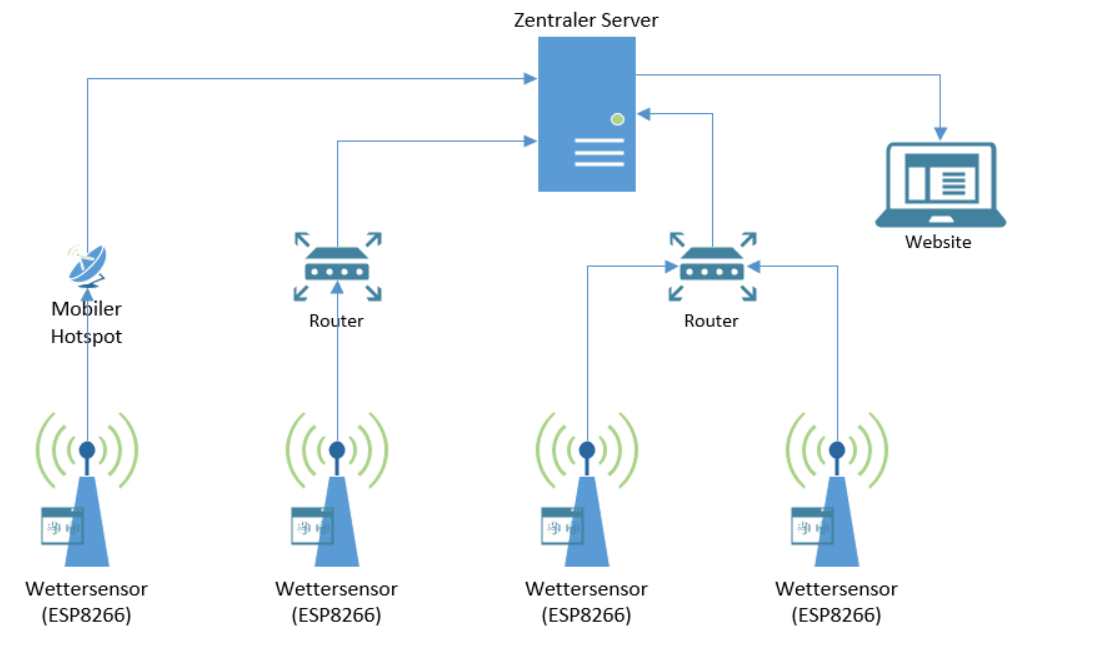
\includegraphics[width=0.7\linewidth]{img/projektkomponenten}
    \caption[Komponenten des Gesamtsystems]{Komponenten des Gesamtsystems (eigene Darstellung)}
    \label{fig:projektkomponenten}
\end{figure}
\\
%In \autoref{fig:projektkomponenten} ist ein möglicher Aufbau der Projektkomponenten gemäß den Projektanforderungen\footnote{\cite{Wortmann.2020}} dargestellt.
Der \enquote{zentrale Server} besteht aus zwei Modulen, dem \enquote{Backend} sowie dem \enquote{Frontend} welche im Folgenden vorgestellt werden.

\subsection{NodeMCU}
Wie in \autoref{ESP} beschrieben, kommt im Projekt ein NodeMCU Mikrocontroller zum Einsatz.
Auf dem Mikrocontroller erfolgt die Erfassung der Messdaten mit einem BME280-Sensor und der Versand an das Backend.
Bei der Auswahl der Libraries wurde hierbei beachtet, möglichst auf den Anwendungsfall spezifische Libraries zu wählen um die Auslastung des Mikrocontrollers zu minimieren.
Ein geringer Energieverbrauch wird in der Programmierung besonders beachtet.
Dadurch ist die Funktionalität auf das wesentliche beschränkt während trotzdem eine zuverlässige Funktionsweise gewährleistet wird.
Wenn der Mikrocontroller keine Verbindung zum angegebenen WLAN-Netzwerk herstellen kann oder der Server nicht erreichbar ist, werden die Daten gecached und versandt, sobald eine Verbindung hergestellt werden kann.\\
Der Mikrocontroller wird in der Arduino IDE in C++ programmiert.

\subsection{Backend}
Das Backend-Modul des Projekts wird auf dem zentralen Server bereitgestellt.
Das Backend basiert auf der \enquote{Node.js}\footnote{\cite{nodejs}} Runtime in Version 14.4, ist somit in Javascript geschrieben und verwendet eine SQLite-Datenbank in Version 3 für die Speicherung der Daten.
Für die Kommunikation zu den Sensoren und dem Frontend ist eine REST-API vorhanden, die in \autoref{Schnittstellen} näher erläutert wird.\\
Sowohl das Backend als auch das Frontend sind für das Deployment in Docker vorgesehen.
Hierbei ist eine örtliche Trennung zwischen Backend und Frontend möglich. Das Frontend kann auf jeden Server zugreifen, der die API dieses Projekts bereitstellt.

\subsection{Frontend}
Das Frontend-Modul, welches die Weboberfläche bereitstellt, basiert ebenfalls auf \enquote{Node.js} in Version 14.4.
Aufgrund des Projektaufbaus ist es wie oben genannt möglich, das Hosting von Backend und Frontend zu trennen.\\
Für die Bereitstellung des Frontends nutzen wir die durch \enquote{Express}\footnote{\cite{express.2020}} bereitgestellte \enquote{Router}-Library.
Die Darstellung der Messdaten auf der Website erfolgt mit \enquote{Chart.js}\footnote{\cite{chartjs.2020}}.
Die Auswahl eines Zeitraums für die Darstellung eines Intervalls ist mit der Library \enquote{daterangepicker}\footnote{\cite{daterangepicker.2020}} umgesetzt.
Zusätzlich wurde für das Projekt \enquote{Browserify}\footnote{\cite{browserify.2020}} verwendet, um den innerhalb des Browsers ausgeführten Code mithilfe von Node.JS testbar zu machen.
Die HTML- und CSS-Komponenten der Website sind mithilfe von Bootstrap 4 erstellt worden.
Auf die Gestaltung wird in \autoref{GUI-Konzept} näher eingegangen.
